\section{Development}
This section is intended to address guidelines for the development and quality assurance of code that will result in the end product. The project is set up with TypeScript. The client (Angular) and the server (Node.js) run in seperate Docker containers and are orchestrated with Docker-compose.

\subsection{Code conventions}
As the project is set up with TypeScript (TS), \href{https://google.github.io/styleguide/tsguide.html}{Google's TypeScript Style Guide} must be followed for all TS code.

Names for functions and variables must be written with camelCase and be self-explanatory. Names generated by Angular should not be changed.

\subsection{Workflow}
The project uses a form of feature branch workflow. Feature branches are merged with a development branch, never directly to the main branch. Once the code has passed testing on the develop branch, it can be merged into the main branch by an authorized manager.

\begin{figure}[H]
    \centering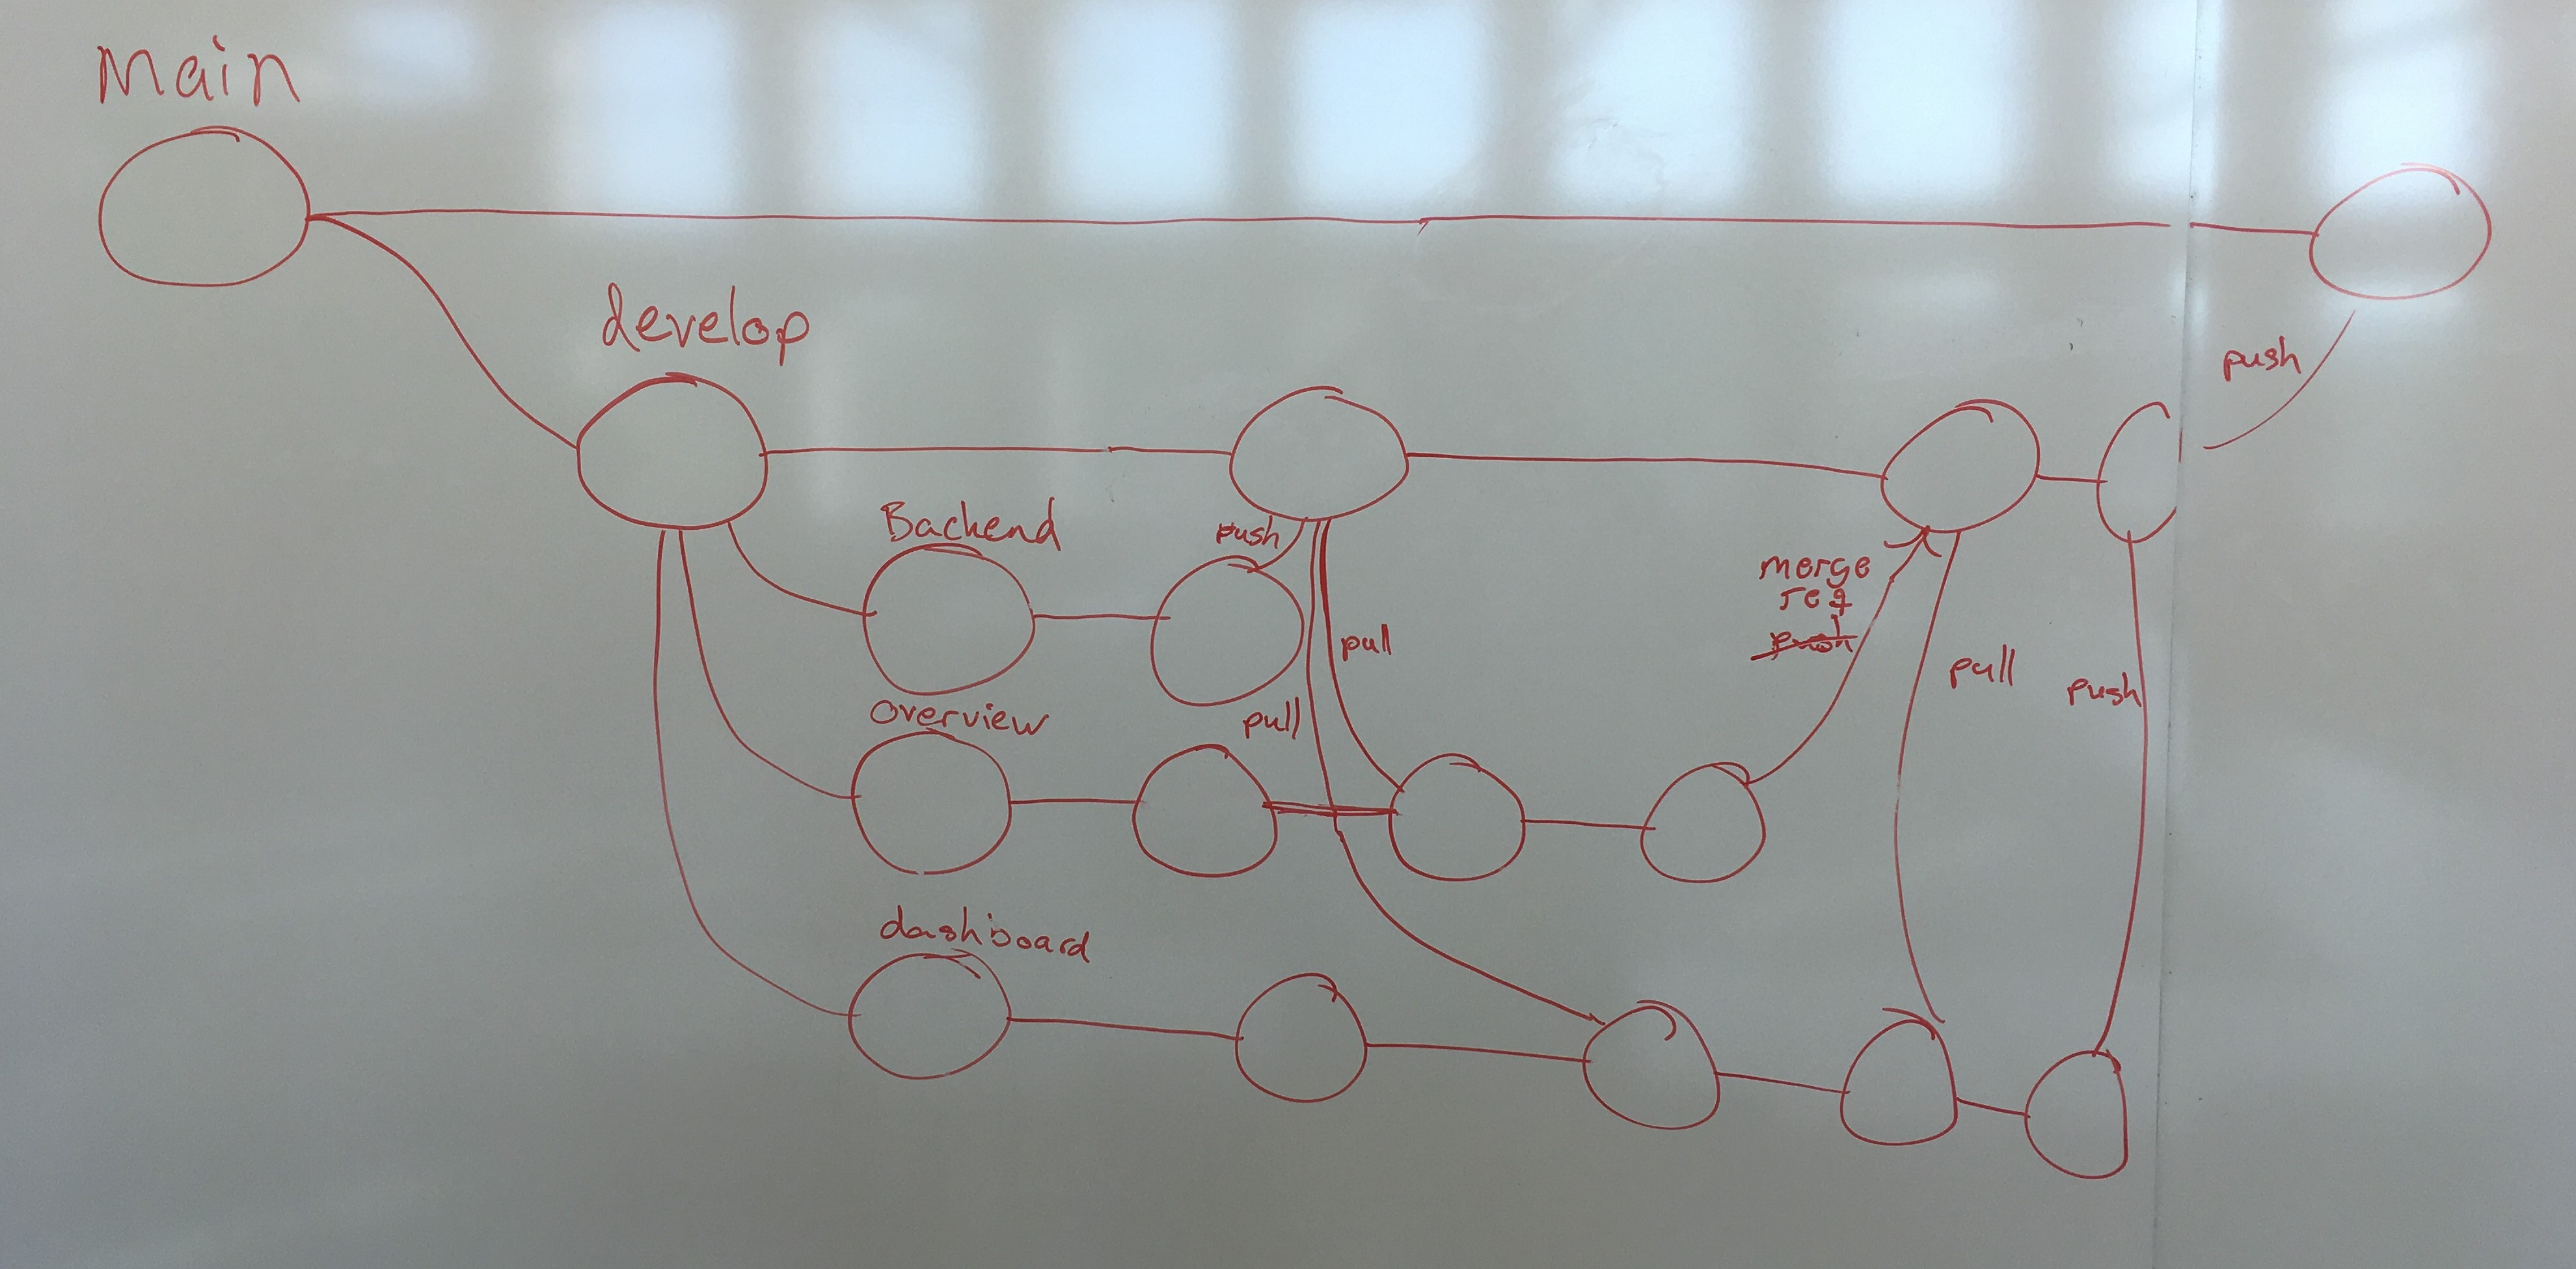
\includegraphics[width=1\linewidth]{figures/workflow-sketch.jpg}
    \caption{Sketch of current workflow on GitLab.}
    \label{fig:workflow}
\end{figure}

\noindent There are five long-lived branches:
\begin{itemize}
\item \emph{main} - Is updated each iteration, code on this branch must be able to be shown to the customer. Members are only allowed to pull code from develop to main.
\item \emph{develop} - The intermediate branch where code from backend, overview and dashboard should be merged to. Code on this branch must be ready to be tested (integration, regression and acceptance testing). Here it is fine to have some bugs.
\item \emph{backend} - CFT1
\item \emph{overview} - CFT2
\item \emph{dashboard} - CFT3
\end{itemize}

\noindent From the three cross-functional team branches, smaller feature branches shall be created. These smaller branches are not supposed to live longer than maximum two days, this is to enable continuous integration. When these smaller branches are merged to their respective CFT branch, peer-reviews must be made (see subsection \ref{subsec:reviews} below). 
All merge requests must be approved according to the set guidelines before it is merged.

\subsection{Software reviews}
\label{subsec:reviews}
In addition to regular discussion of code between developers, software reviews take place in connection with each merge from feature branches to the development branch. The software review must follow a set protocol in GitLab, the guidelines can be found in \href{https://gitlab.liu.se/tddc88-company-1-2021/deploy/-/blob/develop/README.md}{the README-file on GitLab}. In merge requests, the related requirement must be declared as well as what new features have added, the expected behavior of these and what to test.

The reviews are done by a project member who has not developed the code themselves within two working days of when the merge request was posted. The review must not exceed one hour. For merges to the main branch, the review must be done by the project architect.

\subsection{Bug-tracking system}
GitLab is used for bug-tracking. Bugs will be listed, classified and get unique ID as issues in \href{https://gitlab.liu.se/tddc88-company-1-2021/deploy/-/issues}{the Issues tab of the company GitLab}. \emph{Further guidelines for bug-tracking will be found on the company GitLab.}

\subsection{Version handling}
GitLab is used for version handling. Work needs to be commited at least daily when working on features but the goal is to commit after each working addition to the code. Commits must be tagged with what kind of commit it is (see \href{https://gitlab.liu.se/tddc88-company-1-2021/deploy/-/blob/develop/README.md}{the section Semantic Commit Messages in the README-file on GitLab}).

\subsection{Documentation}
The Technical Writer and the involved developers document the code produced at module level. The documentation includes descriptions of which inputs are handled, which functions are used, which inputs are given and how they work together with the rest of the system.
